\subsubsection{Object Model}
Our object model shows the main display of the program we intend to build. 
On the frontend the user gets to view the different posts in an audit log 
with the functionality of being able to add another post which on the backend 
is verified onto the blockchain. All our blocks contain a date,
data and hash so that we can locate them on the blockchain 
and add more to the blockchain being able to verify their validity.
\begin{figure}[h]
\centering % centre is you want
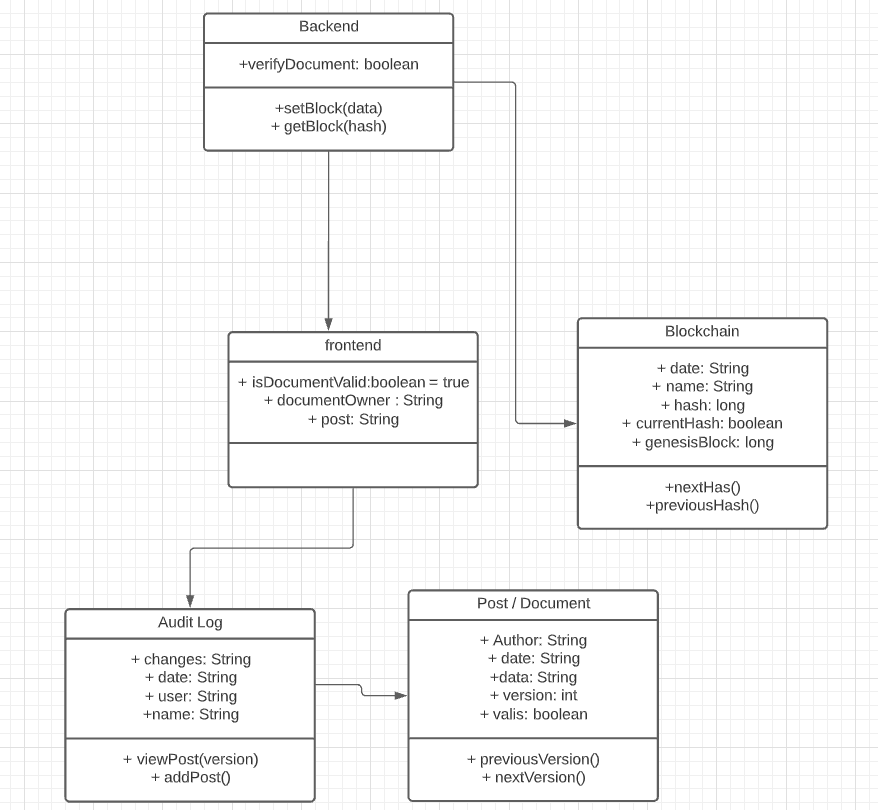
\includegraphics[scale=0.65]{object-model} % To learn more go to: https://www.overleaf.com/learn/latex/Inserting_Images 
\caption{Object model of the system}
\label{fig: object-model} % Can be used with function \ref{fig: passion-fruit-flower} to reference to image
\end{figure}
